\documentclass[aspectratio=169,xcolor=dvipsnames]{beamer}
\usepackage{hyperref}
\usepackage{graphicx, animate}
\usepackage{booktabs}
\usepackage{bbm} % indicatrices

\usetheme{SimpleDarkBlue}

\newcommand{\bdOne}{\mathbbm{1}}

\title{Stratification: Monte Carlo and Simulation}
\author{
    Alban \textsc{Géron}, \\
    Arnaud \textsc{Barrat}, \\
    Camille \textsc{Legrée-Hagbarth}, \\
    Tristan \textsc{Fabre}
}
\date{April 29\textsuperscript{th}, 2025}



\begin{document}
    \begin{frame}
        \titlepage
    \end{frame}

    \begin{frame}{Introduction}
        % @Arnaud ? jsp trop ce que tu voulais mettre pour le benchmark
    \end{frame}

    \begin{frame}{Problem}
        We aim to estimate the integral
        %
        \[I = \int_{[0, 1]^d} f(u) du\]
        %
        where, for all $u = (u_1, \dots, u_d) \in [0, 1]^d$,
        %
        \[f(u) = \cos\left(2 \pi \left(\frac{1}{d} \sum_{i = 1}^d u_i - \frac{1}{2}\right)\right)\]
    \end{frame}

    \begin{frame}{Summary}
        \tableofcontents
    \end{frame}

    \section{Estimation methods used to solve the problem (Monte-Carlo, quasi-Monte-Carlo)}

    \begin{frame}{Monte-Carlo}
        \begin{itemize}
            \item<1-> Notice that $I = \mathbb{E}[f(U)]$, where $U \sim \mathcal{U}([0, 1]^d)$.

            \item<2-> Thus, following Monte-Carlo's method, we approximate such an expectation by
            %
            \[\frac{1}{N} \sum_{n = 1}^N f(U_n)\]
            %
            where $N$ is a large integer and the $U_n$'s are $N$ i.i.d. random vectors uniformly distributed on $[0, 1]^d$.
        \end{itemize}
    \end{frame}

    \begin{frame}{Quasi-Monte-Carlo}
        \begin{itemize}
            \item<1-> In the course's slides, quasi-Monte-Carlo has been proven to be more efficient in terms of computation than Monte-Carlo, under weak assumptions.

            \item<2-> Again, we approximate $I = \mathbb{E}[f(U)]$ by an empirical mean of the form $\frac{1}{N} \sum_{n = 1}^N f(U_n)$. However here the $U_n$'s are generated in the set $\mathcal G = \left\{\frac{1}{2N}, \frac{3}{2N}, \dots, \frac{2N - 1}{2N}\right\}^d$ under the condition \eqref{eq:cdC}:
            %
            \begin{equation}
                \alert{\text{each one of the points } U_1, \dots, U_N \text{ falls on exactly one strip of the set } \mathcal G} \tag{C}\label{eq:cdC}
            \end{equation}

            \item<3-> For $d = 2$: the condition \eqref{eq:cdC} means that there is exactly one point in each line and each column:
            %
            \begin{center}
                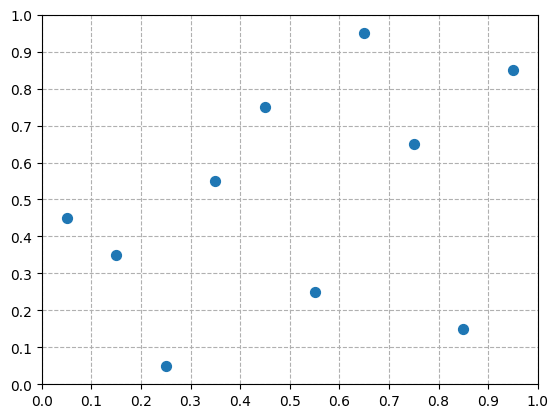
\includegraphics[width=0.3\textwidth]{points2.png}
            \end{center}
        \end{itemize}
    \end{frame}

    \begin{frame}{Quasi-Monte-Carlo ($d = 3$)}
        \begin{itemize}
            \item For $d = 3$: % animation stylée mais je la commente car elle décuple le temps de compilation
            %
            % \begin{center}
            %     \animategraphics[autoplay,loop,width=0.6\linewidth]{10}{gif_frames/frame_}{000}{179}
            % \end{center}
        \end{itemize}
    \end{frame}

    \begin{frame}{Quasi-Monte-Carlo (formalization)}
        \begin{itemize}
            \item<1-> \eqref{eq:cdC} boils down to generating a $d$-dimensional table $M = (m_{i_1, \dots, i_d}) \in \mathbb{R}^{N^d}$ such that
            %
            \[m_{i_1, \dots, i_d} = \bdOne_{i_1 = \sigma_2(i_2) = \cdots = \sigma_d(i_d)}, \qquad \forall (i_1, \dots, i_d) \in \{0, 1, \dots, N - 1\}^d\]
            %
            where $\sigma_2, \dots, \sigma_d$ are $d - 1$ permutations of $\{0, 1, \dots, N - 1\}$.

            \item<2-> \texttt{numpy.random.permutation([0, 1, ..., N - 1])}: an permutation of $\{0, 1, \dots, N - 1\}$ (unidimensional array of size $N$) generated uniformly on the (finite) set $\mathfrak{S}(\{0, 1, \dots, N - 1\})$.

            \item<3-> Then, we get the coordinates of the `ones' as follows. For all $i_1 = 0, 1, \dots, N - 1$, we get \textbf{the only `$1$' that has coordinate $i_1$ on the first axis}, whose coordinates are
            %
            \[i_1, \sigma_2^{-1}(i_1), \dots, \sigma_d^{-1}(i_1)\]
        \end{itemize}
    \end{frame}

    \section{Implementation of unbiased estimators using N. \textsc{Chopin}'s paper}

    \begin{frame}{Haber's Estimators: Intuition}
        Let \( f : [0,1]^d \to \mathbb{R} \) be integrable. We want to approximate:
        \[
        I(f) := \int_{[0,1]^d} f(u) \, du
        \]
        \textbf{Idea:} Use a stratified sampling scheme based on a regular grid:
        $$\begin{aligned} \mathfrak{C}_k := &\left\{\left(\frac{2j_1 + 1}{2k}, \dots, \frac{2j_d + 1}{2k}\right) \quad \text{s.t.} \quad (j_1, \dots, j_d) \in \{0, 1, \dots, k - 1\}^d\right\} \\ = &\left\{\frac{1}{2k}, \frac{3}{2k}, \dots, \frac{2k - 1}{2k}\right\}^d \end{aligned}$$
        where $d$ is the dimension of the hypercube of size $[0,1]^d$ and $k$ the level of stratification. Consequently, this define a grid of size $k^d$.  
        \vspace{1em}

        Each point \( c \in \mathfrak{C}_k \) is the centre of a cube of side \( \frac{1}{k} \).  
        \vspace{1em}
        %%%%%%%%%%% TODO : image
        \vspace{0.5em}
        \textbf{Goal:} Reduce variance compared to naive Monte Carlo using stratification and local symmetry.
    
            
    \end{frame}

    \begin{frame}{Haber's Estimators: Goals}
        \begin{enumerate}
            \item Reduce the variance
            \item ...
            \item ...
        \end{enumerate}


    \end{frame}

    \begin{frame}{Comparison: Haber vs. Quasi-Monte Carlo}
        \textbf{Quasi-Monte Carlo (QMC):}
        \begin{itemize}
            \item Uses low-discrepancy sequences (e.g., Sobol) to cover \([0,1]^d\) more uniformly than random sampling.
            \item Deterministic and achieves convergence rates close to \( \mathcal{O}(1/N) \) for smooth functions.
        \end{itemize}
        
        \textbf{Haber Estimators:}
        \begin{itemize}
            \item Use regular grid stratification \( \mathfrak{C}_k \) with random perturbations.
            \item Preserve randomness (unbiased estimators).
            \item Order 2 estimator incorporates local symmetry → reduced bias and variance.
        \end{itemize}
        
        \vspace{1em}
        \textbf{Comparison:}
        \begin{itemize}
            \item QMC: low-discrepancy but deterministic.
            \item Haber: randomized, better than MC, less optimal than QMC on smooth functions.
            \item Haber can be preferable in stochastic or noisy settings (where QMC struggles).
        \end{itemize}
    \end{frame}

    %%%%% mettre à la fin et inclure un tableau où on compare les estimations et la variance pour différentes valeurs de k, d et N

    \begin{frame}{Haber's estimator of order 1}
        \begin{itemize}
            \item Haber's first estimator is defined by
            $$\hat{I}_{1,k}(f) := \frac{1}{k^d} \sum_{c \in \mathfrak{C}_k} f(c + U_c), \quad U_c \sim \mathcal{U}\left(\left[-\frac{1}{2k}, \frac{1}{2k}\right]^d\right)$$
            \item Instead of randomly dropping samples everywhere, this method \textbf{ensures a uniform spatial coverage} by stratifying the domain into small subcubes.
        
            \item The perturbation $U_c$ inside each hypercube introduces \textbf{randomness}, allowing us to sample the function $f$ without relying solely on the midpoints (which could be biased).
        \end{itemize}
    
        %%%%%%%%%%%%%%%%% ajouter image + expliquer comment ca réduit la variance
    \end{frame}

    \begin{frame}{Haber's estimator of order 2}
        Let
        $$g_c(u) := \frac{f(c + u) + f(c - u)}{2}$$

        Haber's second estimator is the following:
        $$\hat{I}_{2,k}(f) := \frac{1}{k^d} \sum_{c \in \mathfrak{C}_k} g_c(U_c), \quad U_c \sim \mathcal{U}\left(\left[-\frac{1}{2k}, \frac{1}{2k}\right]^d\right)$$
    \end{frame}
    %%%%%%%%%%%%%%%%% ajouter image + expliquer comment ca réduit la variance + expliquer l'intuition

    %%%%%%% limites du modèles
    \section{Implementation of importance sampling methods}

    \begin{frame}{Frame Title}
        
    \end{frame}
\end{document}